\documentclass{article}

% if you need to pass options to natbib, use, e.g.:
% \usepackage[sectionbib]{natbib}
    \PassOptionsToPackage{numbers}{natbib}
% before loading neurips_2019

% ready for submission
% \usepackage{neurips_2019}

% to compile a preprint version, e.g., for submission to arXiv, add add the
% [preprint] option:
%     \usepackage[preprint]{neurips_2019}

% to compile a camera-ready version, add the [final] option, e.g.:
\usepackage[final]{neurips}

% to avoid loading the natbib package, add option nonatbib:
    % \usepackage[nonatbib]{neurips_2019}
\usepackage{}
\usepackage[utf8]{inputenc} % allow utf-8 input
\usepackage[T1]{fontenc}    % use 8-bit T1 fonts
\usepackage{url}            % simple URL typesetting
\usepackage{booktabs}       % professional-quality tables
\usepackage{amsfonts}       % blackboard math symbols
\usepackage{nicefrac}       % compact symbols for 1/2, etc.
\usepackage{microtype}      % microtypography
\usepackage{tikz}
\usepackage{booktabs}
\usepackage{multirow}
\usepackage{makecell}
\usepackage{multicol}
\usepackage{tabularx}
\usepackage{subcaption}

\newcolumntype{R}{>{\raggedleft\arraybackslash}X}
\newcolumntype{L}{>{\raggedright\arraybackslash}X}


\usetikzlibrary{shapes.geometric, arrows}
\usepackage[colorlinks=true]{hyperref} % hyperlinks

\title{Space Efficient Deep Learned Inverted Index Representation}

% The \author macro works with any number of authors. There are two commands
% used to separate the names and addresses of multiple authors: \And and \AND.
%
% Using \And between authors leaves it to LaTeX to determine where to break the
% lines. Using \AND forces a line break at that point. So, if LaTeX puts 3 of 4
% authors names on the first line, and the last on the second line, try using
% \AND instead of \And before the third author name.

\author{%
  Antonio Mallia \\
  Tandon School of Engineering\\
  New York University\\
  \texttt{antonio.mallia@nyu.edu} \\
  % examples of more authors
   \And
    Yair Schiff \\
    Courant Institute\\
    New York University\\
    \texttt{yair.schiff@nyu.edu} \\
    \And 
    Yves Greatti \\
    Courant Institute\\
    New York University\\
    \texttt{yves.greatti@nyu.edu}
}

\begin{document}

\maketitle

\begin{abstract}
An inverted index is the basic data structure used in most current, large-scale information retrieval systems.
Many compression techniques for inverted indexes have been studied in the past, with some reaching significant compression ratios, while preserving query time efficiency.
In this project, we aim to use Deep Learning models to replace the index structure, resulting in better compression of the inverted index. We present results that indicate that with further refinement this learned inverted index structure can reduce memory requirements and provide a novel approach to learned compression.
\end{abstract}

\section{Introduction}\label{sec:intro}
An inverted index is the key data structure used in most large-scale text search systems.
For a corpus of documents, a list of unique terms is extracted and the documents are each given a unique integer document ID.
For each unique term, a sorted sequences of integers, known as a \textit{posting list} is created.
A posting list is a sequence of the document IDs that contain the corresponding term.
Given the large collections indexed by current search engines, even a single node of a large search cluster typically contains many billions of integers.
Thus, space efficiency is crucial to maintaining acceptable query response times, which motivates the use of specialized index compression techniques.

To this end, our project explores the application of Deep Learning (DL) models in `learning' the inverted index.
Recently, other attempts have been made \cite{OosterhuisCR18} along these lines, but they approach the problem in a different way. The authors of \citet{OosterhuisCR18} focus on learning an inverted index by using models that act as learned Bloom-filters, in order to perform conjunctive Boolean querying.
Our proposal provides a more flexible solution to this quite limiting case.


The goal of our work is to build lightweight neural networks that can accurately memorize posting lists with the intention that saving the model weights for a posting list will be less memory intensive than saving the posting list itself.
In addition to saving the weights, we store the errors between predicted document IDs and the true document IDs of a posting list, so that at retrieval time, the posting list is recreated with perfect fidelity.
A similar approach is proposed by \citet{GPU}, but the authors there do not make use of any DL models to generate the approximation of the distribution.
Rather, they use simple linear regression to leverage the significant linear characteristics expressed by posting lists.
Although this purely linear structure is true for some posting lists, we believe that this solution does not generalize well to entire inverted indexes and believe that DL methods have greater potential to beat other compression techniques.

This paper is organized as follows.
Section \ref{sec:related_work} below details the past research motivating our project.
In Section \ref{sec:methodology}, we explain the various approaches that we employ, and in Section \ref{sec:results}, we highlight results observed from our experiments.
Finally, Section \ref{sec:conclusions} provides concluding remarks and proposals for extending our work.

\section{Related Work}\label{sec:related_work}
The main motivation for our work is that of Kraska et al. \cite{Kraska2018}, which recently proposed a novel and somewhat surprising insight of approaching indexing as a learning problem.
The authors suggest that index structures can be interpreted as functional mappings that can be learned by Machine Learning models. 
For example, a B-Tree-Index can be seen as a model that maps a key to the position of a record within a sorted array.
The benefit of learned index structures is that they require less memory and can be evaluated substantially faster than their traditional counterparts.

\subsection{Compression Methods}
We now briefly outline the compression methods that are typically employed to compress an inverted index.
\textbf{OptPFor} \cite{OptPForDelta} encodes a large number of integers (say, 64 or 128) at a time by choosing an integer $k$ such that most (e.g. 90\%) of the integers can be encoded in $k$ bits.
The \textbf{Simple-8b} \cite{simple8b} technique tries to pack as many numbers as possible into one machine word to achieve faster decoding.
\citet{SIMD-BP128} proposed a bit-packing method that uses SIMD instructions.
The algorithm, called \textbf{SIMD-BP128}, packs 128 consecutive integers into as few 128-bit words as possible.
The 16-byte selectors are stored in groups of 16 to fully utilize 128-bit SIMD reads and writes.

\section{Methodology}\label{sec:methodology}
We aim to expand results obtained by Kraska et al. \cite{Kraska2018} to the compression of inverted index.
That is, rather than maintaining $n$ posting lists, where $n$ corresponds to the number of unique terms in the corpus, the goal is to store the model weights that can reproduce these lists and that have a lighter memory footprint than the lists themselves.

To achieve this goal we try several approaches.
However, it is worth noting that all of our approaches are regression techniques.
The reason that we cannot use classification is because the number of unique document IDs in a corpus is typically large.
Therefore, inputs to a softmax layer that would be used to classify the outputs of our networks as one of the documents in the corpus would contain too many weights and defeat the purpose of the this project.

Turning now to the approaches we employ, given the sequential nature of each posting list we first experiment with recurrent neural nets (RNNs), which have been shown to have the necessary capacity to learn short-term and long-term dependencies in natural signals.
We specifically test LSTM and GRU models.
Within our RNN modeling, we attempt to learn a `global' model, i.e. one model for the entire inverted index, and many `local' models, i.e. $n$ unique models - one per term ID.
For both the global and local axes, we also attempt approaches that we call `index2doc' and `doc2doc'.
For `index2doc' we provide the RNN cells the indices of the elements of a posting list.
For `doc2doc' we provide the previous document ID and predict the next one in the sequence.

In addition to the more complex recurrent models, we experiment with simpler feed-forward networks.
For the feed-forward models, we explore only the `index2doc' method.
Starting from wide one-hidden-layer networks that overfit each posting list and memorize document IDs perfectly, we try several architecture sizes, in order to balance model memory footprint and accuracy.
Additionally, since the feed-forward models cannot capture longer term dependencies, rather than learning one model per posting list, we break each list into batches (e.g. of size 32, 64, etc.) and train one model per batch.

We also try to learn the optimal segmentation of the posting list, rather than uniformly splitting them into batches.
That is, we segment the posting lists into chunks of document IDs that should be easier to learn.
To perform this intra-posting list clustering we use the k-means algorithm.
This design introduces a new hyper-parameter, which is the number of clusters of document IDs per posting list. Our experiments yield that the optimal number of clusters is dictated by the capacity of the neural network model we use, which we empirically found, to be no more than twenty document IDs per clusters. 

Finally, we implement the algorithm described in  Kraska et al. \cite{Kraska2018}, which uses a variable number of neural network models trained on different ranges of document IDs of a posting list. 
Training is performed hierarchically.
The top of the hierarchy contains a model that trains on the entire posting list.
If this model is not able to achieve a loss below a certain threshold, the posting list is broken into batches of equal size and a new model is trained on each batch.
This continues until either the depth is maximized or the loss threshold is met.
This algorithm is tested using various hyperparameters, such as hierarchy depth and number of hidden layers per neural network.

For all of our models, we compress the weights using model quantization.
For example, the weights of a one-hidden-layer neural network are quantized into a several bytes depending on whether or not biases are included (ranging from 16 bytes to 24 bytes for 3 hidden unit networks).

\section{Results}\label{sec:results}
Unfortunately due to the time constraints of the project we were not able to optimize all of the various  models and approaches detailed above.
The experimental results noted below therefore focus on the easier to train shallow feed-forward networks that were applied to batches of document IDs and full posting lists.
Nevertheless, even with these simpler networks, we find promising results that point to the efficacy of learning inverted indexes.

We begin by demonstrating that a large network can easily overfit and memorize a full posting list.
However, given the goal of this work is to reduce memory footprint, we were constrained to smaller and shallower networks which perform less accurately when applied to entire posting lists.
This trade-off is highlighted in Figure \ref{fig:perfect_vs_shallow}.
\begin{figure}
\centering
\begin{subfigure}{0.5\textwidth}
    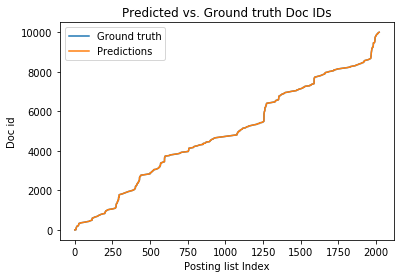
\includegraphics[width=\textwidth]{graphics/perfect.png}
    \label{fig:batch1}
\end{subfigure}%
\begin{subfigure}{.5\textwidth}
    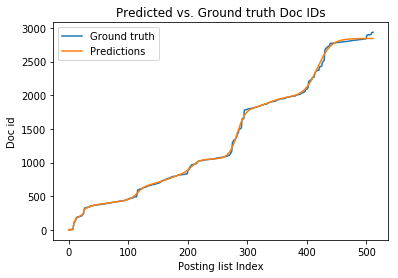
\includegraphics[width=\textwidth]{graphics/shallow.png}
    \label{fig:batch2}
\end{subfigure}%
\caption{(a) The ideal network with near zero loss (b) The shallow network with some significant errors for certain document IDs.}
\label{fig:perfect_vs_shallow}
\end{figure}

To minimize larger errors, we break the posting list into fixed batch sizes. Figure \ref{fig:batch_learning} demonstrates that using lightweight networks on these batches of document IDs yields high accuracy predictions, which bodes well for the application of neural networks to learning inverted indexes.
\begin{figure}
\centering
\begin{subfigure}{0.5\textwidth}
    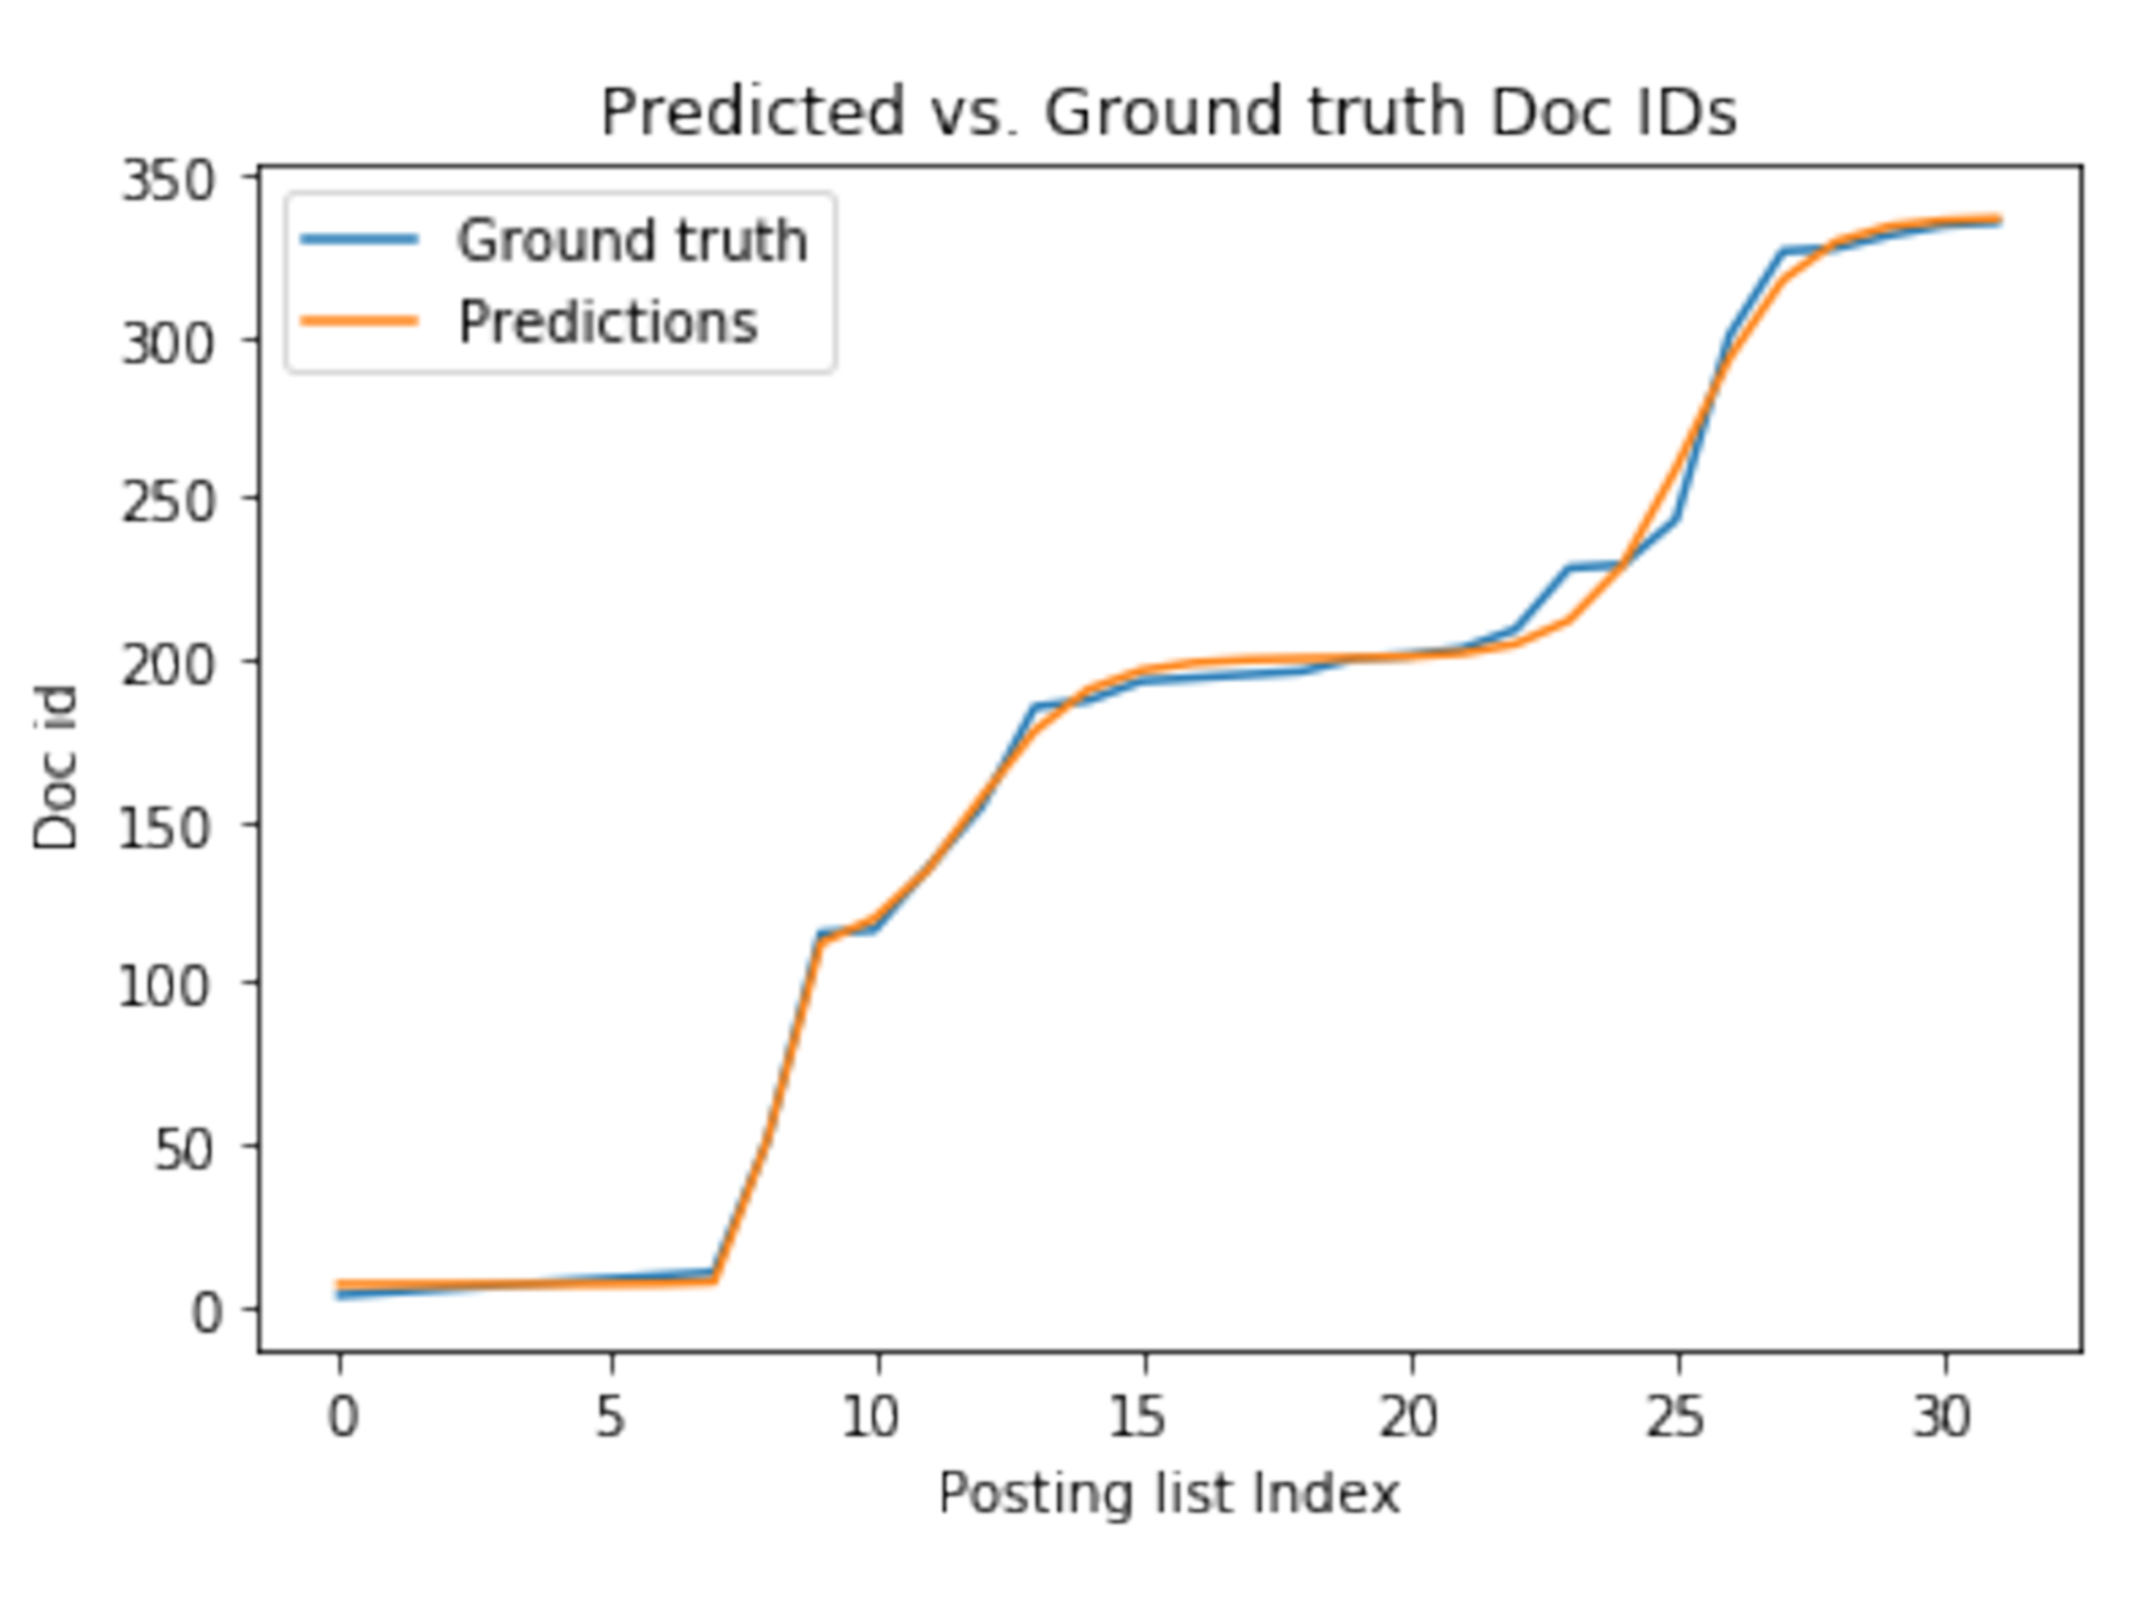
\includegraphics[width=\textwidth]{graphics/image1.pdf}
    \caption{}
    \label{fig:batch_1}
\end{subfigure}%
\begin{subfigure}{.5\textwidth}
    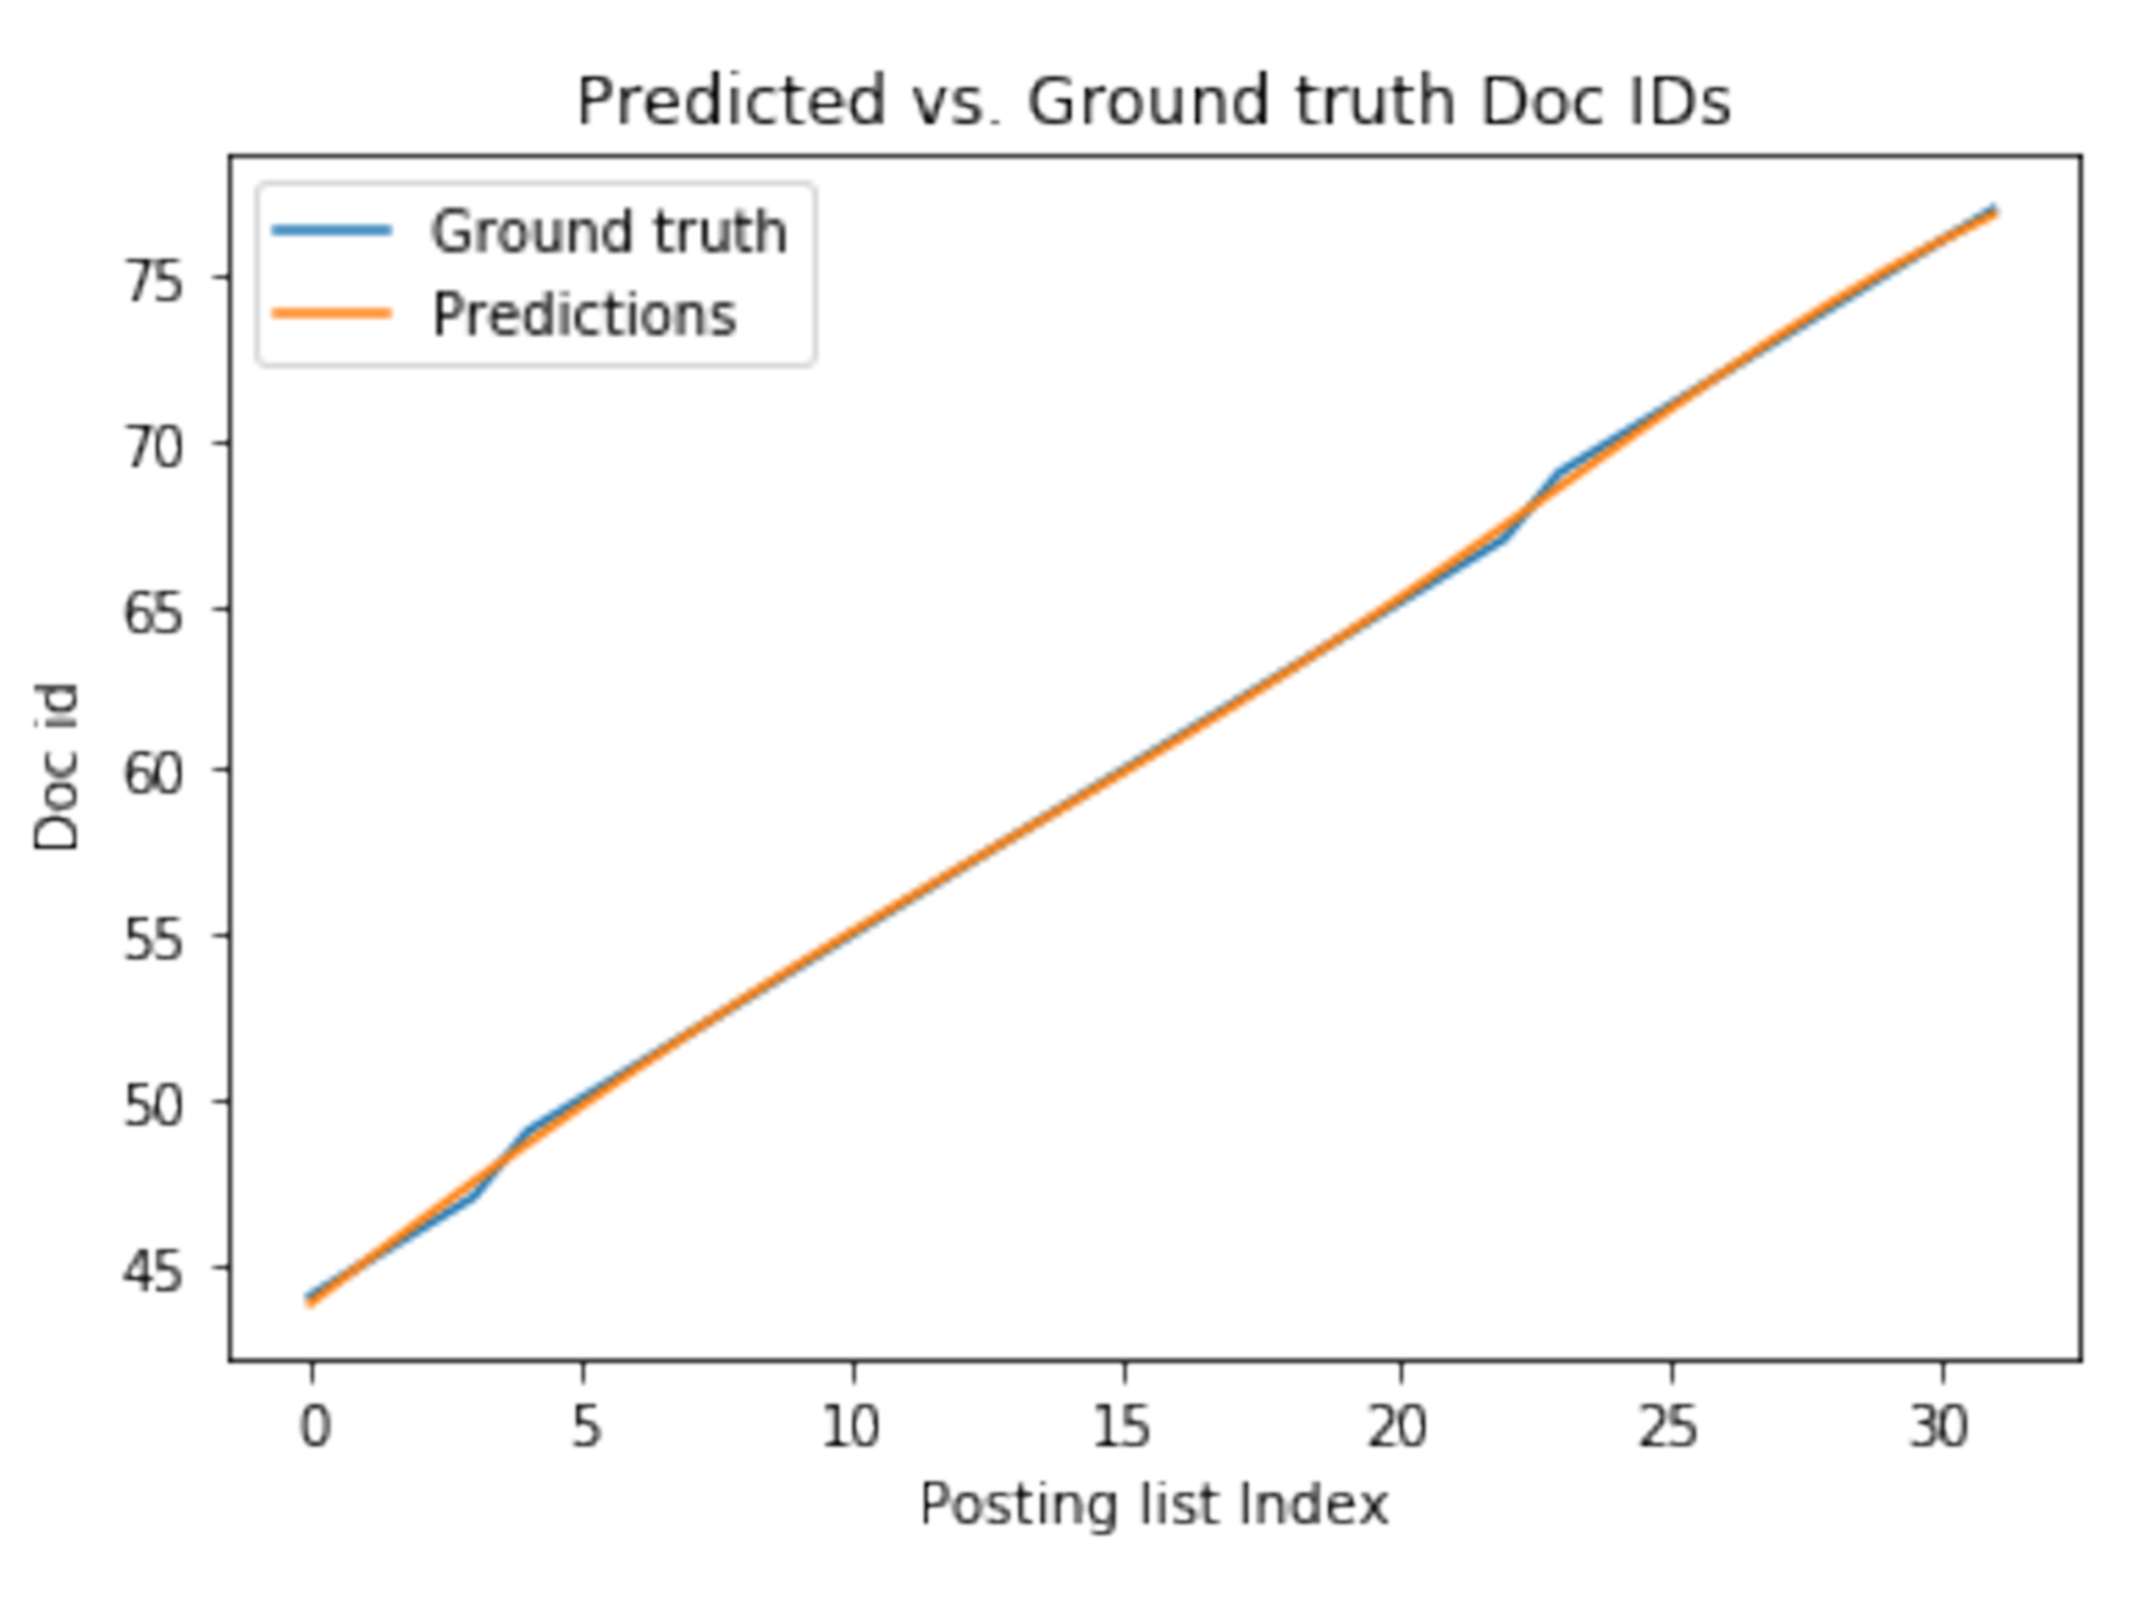
\includegraphics[width=\textwidth]{graphics/image2.pdf}
    \caption{}
    \label{fig:batch_2}
\end{subfigure}%
\caption{Examples demonstrating the predictive power of shallow networks with few hidden units.
These examples are representative of the accuracy observed across batches}
\label{fig:batch_learning}
\end{figure}

Finally, to truly test our approach against the ultimate goal of reducing memory footprint of representations of the original data structure, we compare bits per document ID of various compression techniques in Table \ref{tab:space} below.
The first column of this table represents the number of bits per document ID required to compress the original inverted index. 
The next two columns show the bits per document ID for storing the errors of our predictions and for storing the errors plus the quantized weights of the models.
The last column highlights how we are able to achieve compression gains utilizing learned indexes.
It should be noted that the results in this table come from applying one model per posting list, where each model consisted of one hidden layer with hidden units equal to length of the posting list divided by 40.
Even with this simple approach we are able to realize memory gains, which indicates that through further refinement and training we could yield even better compression ratios.
\begin{table}
\centering
\begin{tabularx}{\textwidth}{lRRRR}\toprule
        & Compressed posting list & \multicolumn{2}{@{}c@{}}{Our approach} & Ratio \\
        & \tiny{Bits per docID} &  \tiny{Bits per docID (errors)} &   \tiny{Total Bits per Doc ID (accounting for weights)}  &  \tiny{our approach / compressed posting lists} \\\midrule
    OptPFor   & 5.21  & 3.44 & 4.04 & 78\% \\
    SIMD-BP128 & 7.32 &   3.45 & 4.05 & 55\%  \\
    Simple8b    & 6.43 & 2.32 & 2.92& 40\% \\
    \bottomrule \\
\end{tabularx}
  \caption{Average bits per document ID.}\label{tab:space}
\end{table}



\section{Conclusions and Future Work}\label{sec:conclusions}
In this paper, we have shown the potential of applying DL models to improve inverted index representation size.
We have conducted a preliminary, but promising experimental evaluation using shallow feed-forward networks, where multiple models are used to learn a good approximation of the distribution of the document identifiers in each posting list.
Future work will focus on further compressing the learned models by applying integer compression techniques to the quantized weights.
Moreover, we intend to explore the possibility of using a hierarchical ensemble modeling in order to improve predictions, similarly to what has been done by \citet{Kraska2018}. 
Finally, we think that RNNs can be better leveraged to exploit locality and stationary of the inverted index. A single RNN model, or eventually a fixed pool of models, could be able to approximate the entire index capturing global patterns and similarities.

\bibliographystyle{plainnat}
\bibliography{references}

\end{document}
